\section{Multivariate Explorative Analyse}

\begin{defi}{Multivariate Explorative Analyse}
    Mit Hilfe von \emph{multivariaten Verfahren} werden in der multivariaten Statistik mehrere statistische Variablen oder Zufallsvariablen (\emph{Features}) zugleich untersucht.

    In der univariaten Analyse hingegen wird jede Variable einzeln analysiert.
\end{defi}

\begin{defi}{Scatter-Plot}
    TODO
\end{defi}


\begin{defi}{Bubble Chart}
    TODO
\end{defi}

\subsection{Zusammenhangsmaße (Interdependenzmaße)}

\begin{defi}{Pearsons Korrelationskoeffizient}
    Der \emph{Person'sche Korrelationskoeffizient} ist ein Maß für den Grad des linearen Zusammenhangs zwischen zwei Zufallsvariablen.
    Er kann Werte zwischen $-1$ und $+1$ annehmen.

    Bei einem Wert von $+1$ (bzw. $-1$) besteht ein vollständig positiver (bzw. negativer) linearer Zusammenhang zwischen den betrachteten Merkmalen.
    Wenn der Korrelationskoeffizient den Wert $0$ aufweist, hängen die beiden Merkmale überhaupt nicht linear voneinander ab.

    Allerdings können diese ungeachtet dessen in nichtlinearer Weise voneinander abhängen.

    Damit ist der Korrelationskoeffizient kein geeignetes Maß für die (reine) stochastische Abhängigkeit von Merkmalen.

    Der Pearson'sche Korrelationskoeffizient ist definiert durch
    \[
        \rho_{\text{PE}} := \frac{\Cov(X, Y)}{\sigma_X \cdot \sigma_Y} = \frac{\sum_{i=1}^{n}{(x_i - \conj{x})(y_i - \conj{y})}}{\sqrt{\sum_{i=1}^{n}(x_i - \conj{x})^2 \sum_{i=1}^{n}(y_i - \conj{y})^2}}
    \]
\end{defi}

\begin{defi}{Spearmans Korrelationskoeffizient}
    Der \emph{Spearmans'sche Korrelationskoeffizient} entspricht dem Pearson'schen Korrelationskoeffizient, bezieht sich allerdings auf die Ränge der Werte und charakterisiert somit die Stärke des monotonen Zusammenhangs.

    Seien die Werte $x_i$ einer Stichprobe der Größe $n$ des Merkmals $X$ geordnet:
    \[
        x_1 \leq x_2 \leq \ldots \leq x_n
    \]

    Dann ist der Rang eines Wertes definiert als:
    \[
        \rang(x_i) = i
    \]

    Bei identischen Werten ist die Rangvergabe nicht mehr eindeutig und es wird der Durchschnittsrang gebildet.\footnote{D. h.: identischen Werten wird als Rang das arithmetische Mittel der infrage kommenden Ränge zugewiesen.}

    Es gilt also:
    \[
        \rho_{\text{SP}} :=  = \frac{\sum{(\rang(x_i) - \conj{\rang}_X)(\rang(y_i) - \conj{\rang}_Y)}}{\sqrt{\sum(\rang(x_i) - \conj{\rang}_X)^2 \sum(\rang(y_i) - \conj{\rang}_Y)^2}}
    \]

    mit folgenden Mittelwerten der Ränge:
    \[
        \conj{\rang}_X = \frac{1}{n} \sum_{i=1}^{n} \rang(x_i) = \frac{1}{n} \sum_{i=1}^{n} \frac{n+1}{2}
    \]
    \[
        \conj{\rang}_Y = \frac{1}{n} \sum_{i=1}^{n} \rang(y_i) = \frac{1}{n} \sum_{i=1}^{n} \frac{n+1}{2}
    \]
\end{defi}

\begin{bonus}{Pearson vs. Spearman}
    Es gilt:

    Pearson:
    \begin{itemize}
        \item charakterisiert \emph{lineare} Zusammenhänge
        \item nutzbar für Merkmale (Features) auf \emph{metrischem Skalenniveau}\footnote{d. h. Merkmale unterstützen Operationen wie $\neq$, $=$, $>$, $<$, $+$, $-$, $\cdot$, $\div$}
        \item Beispiele: Nettomiete, Alter
    \end{itemize}

    Spearman:
    \begin{itemize}
        \item charakterisiert \emph{monotone} Zusammenhänge
        \item nutzbar für Merkmale (Features) auf \emph{metrischem oder ordinalen Skalenniveau}\footnote{ordinale Merkmale unterstützen Operationen wie $\neq$, $=$, $>$, $<$}
        \item Beispiele: Ränge, Schwierigkeitsgrad von Aufgaben (leicht, mittel, schwer)
    \end{itemize}
\end{bonus}

\begin{defi}{Invarianz von Korrelationskoeffizienten}
    \begin{enumerate}
        \item Beide Korrelationskoeffizienten sind invariant unter \emph{linearer Transformation}.

              Wenn also die Features $X$ und $Y$ linear transformiert werden mit:
              \[
                  \tilde{X} = a_X X + b_X, \quad \tilde{Y} = a_Y Y + b_Y
              \]
              dann gilt für beide Korrelationskoeffizienten:
              \[
                  \rho = \frac{a_X a_Y}{|a_X| |a_Y|} \rho
              \]

              Das Vorzeichen wir bestimmt durch die Vorzeichen der Koeffizienten von $a_X$ und $a_Y$.
        \item Der Spearman'sche Korrelationskoeffizient ist invariant unter \emph{streng monotonen Transformationen}.

              Wenn also die Features $X$ und $Y$ streng monoton transformiert werden mit:\footnote{$g$ und $h$ sind streng monoton wachsende Funktionen.}
              \[
                  \tilde{X} = g(X), \quad \tilde{Y} = h(Y)
              \]
              dann gilt für den Spearman'schen Korrelationskoeffizient:
              \[
                  \rho_{\text{SP}} = \begin{cases}
                      \rho_{\text{SP}}  & \text{falls $g$ und $h$ beide fallen oder beide steigen} \\
                      -\rho_{\text{SP}} & \text{sonst}
                  \end{cases}
              \]
        \item Beide Korrelationskoeffizienten sind invariant unter \emph{Vertauschung der Merkmale}.

              Korrelation ist ein Maß für die Stärke eines Zusammenhangs zwischen $X$ und $Y$.

              \emph{Die Richtung der Wirkung (sofern existent) wird nicht erfasst!}
    \end{enumerate}
\end{defi}

\subsection{Mutual Information}

\begin{defi}{Informationsgehalt}
    Der \emph{Informationsgehalt} $I_k$ für das Eintreffen eines Ereignisses $k$ mit Wahrscheinlichkeit $p_k$ ist:
    \[
        I_k := - \log_2 p_k \qquad (\text{Einheit: bit})
    \]

    Es gilt:
    \begin{itemize}
        \item Je seltener ein Ereignis $k$, desto größer sein Informationsgehalt.
        \item Logarithmus erleichtert das Rechnen mit Informationsgehalten.
        \item $I_k \geq 0$, da $p_k \in [0, 1]$
        \item Wahl einer anderen Basis des Logarithmus verändert nur die Einheit, in der Informationsgehalt gemessen wird
    \end{itemize}
\end{defi}

\begin{defi}{Entropie}
    Der mittlere Informationsgehalt eines Ereignisses (Ausgangs) eines Zufallsexperiments mit Zufallsvariable $X$ heißt \emph{Entropie} $H(X)$.
    \footnote{auch: Shannon-Entropie, Gibbs-Boltzmann-Entropie}

    \[
        H(X) := \Mean(I) = - \sum_{k=1}^C p_k \log_2 p_k \qquad \text{mit} \ 0 \log_2 0 = 0
    \]

    Die Entropie von $X$ unter der Bedingung des Auftretens eines Wertes $y_j$:
    \[
        H(X \mid y_j) = - \sum_{i} p(x_i \mid y_j) \log_2 p(x_i \mid y_j)
    \]
\end{defi}

\begin{defi}{Bedingte Entropie}
    Der mittlere Informationsgehalt eines Ergebnisses einer Zufallsvariablen $X$ unter der Bedingung, dass der Wert einer Zufallsvariablen $Y$ bekannt ist, heißt \emph{bedingte Entropie} $H(X \mid Y)$.
    \begin{alignat*}{1}
        H(X \mid Y) & = - \sum_{j} p(y_j) H(X \mid Y = y_j)                                              \\
                    & = - \sum_{j} p(y_j) \left( \sum_{i} p(x_i \mid y_j) \log_2 p(x_i \mid y_j) \right) \\
                    & = - \sum_{j} p(x_i, y_j) \log_2 \frac{p(x_i, y_j)}{p(y_j)}
    \end{alignat*}
\end{defi}

\begin{defi}{Mutual Information}
    \emph{Mutual Information} basiert auf Konzepten aus der Informationstheorie.

    Die Abnahme des mittleren Informationsgehalts eines Ergebnisses der Zufallsvariablen $X$ durch Kenntnis des Ergebnisses einer Zufallsvariablen $Y$ heißt \emph{Mutual Information}.
    \[
        \IG(X, Y) = H(X) - H(X \mid Y)
    \]

    Mutual Information ist auch unter der Bezeichnung \emph{Information Gain} (im Kontext von Bäumen) bekannt.

    \begin{center}
        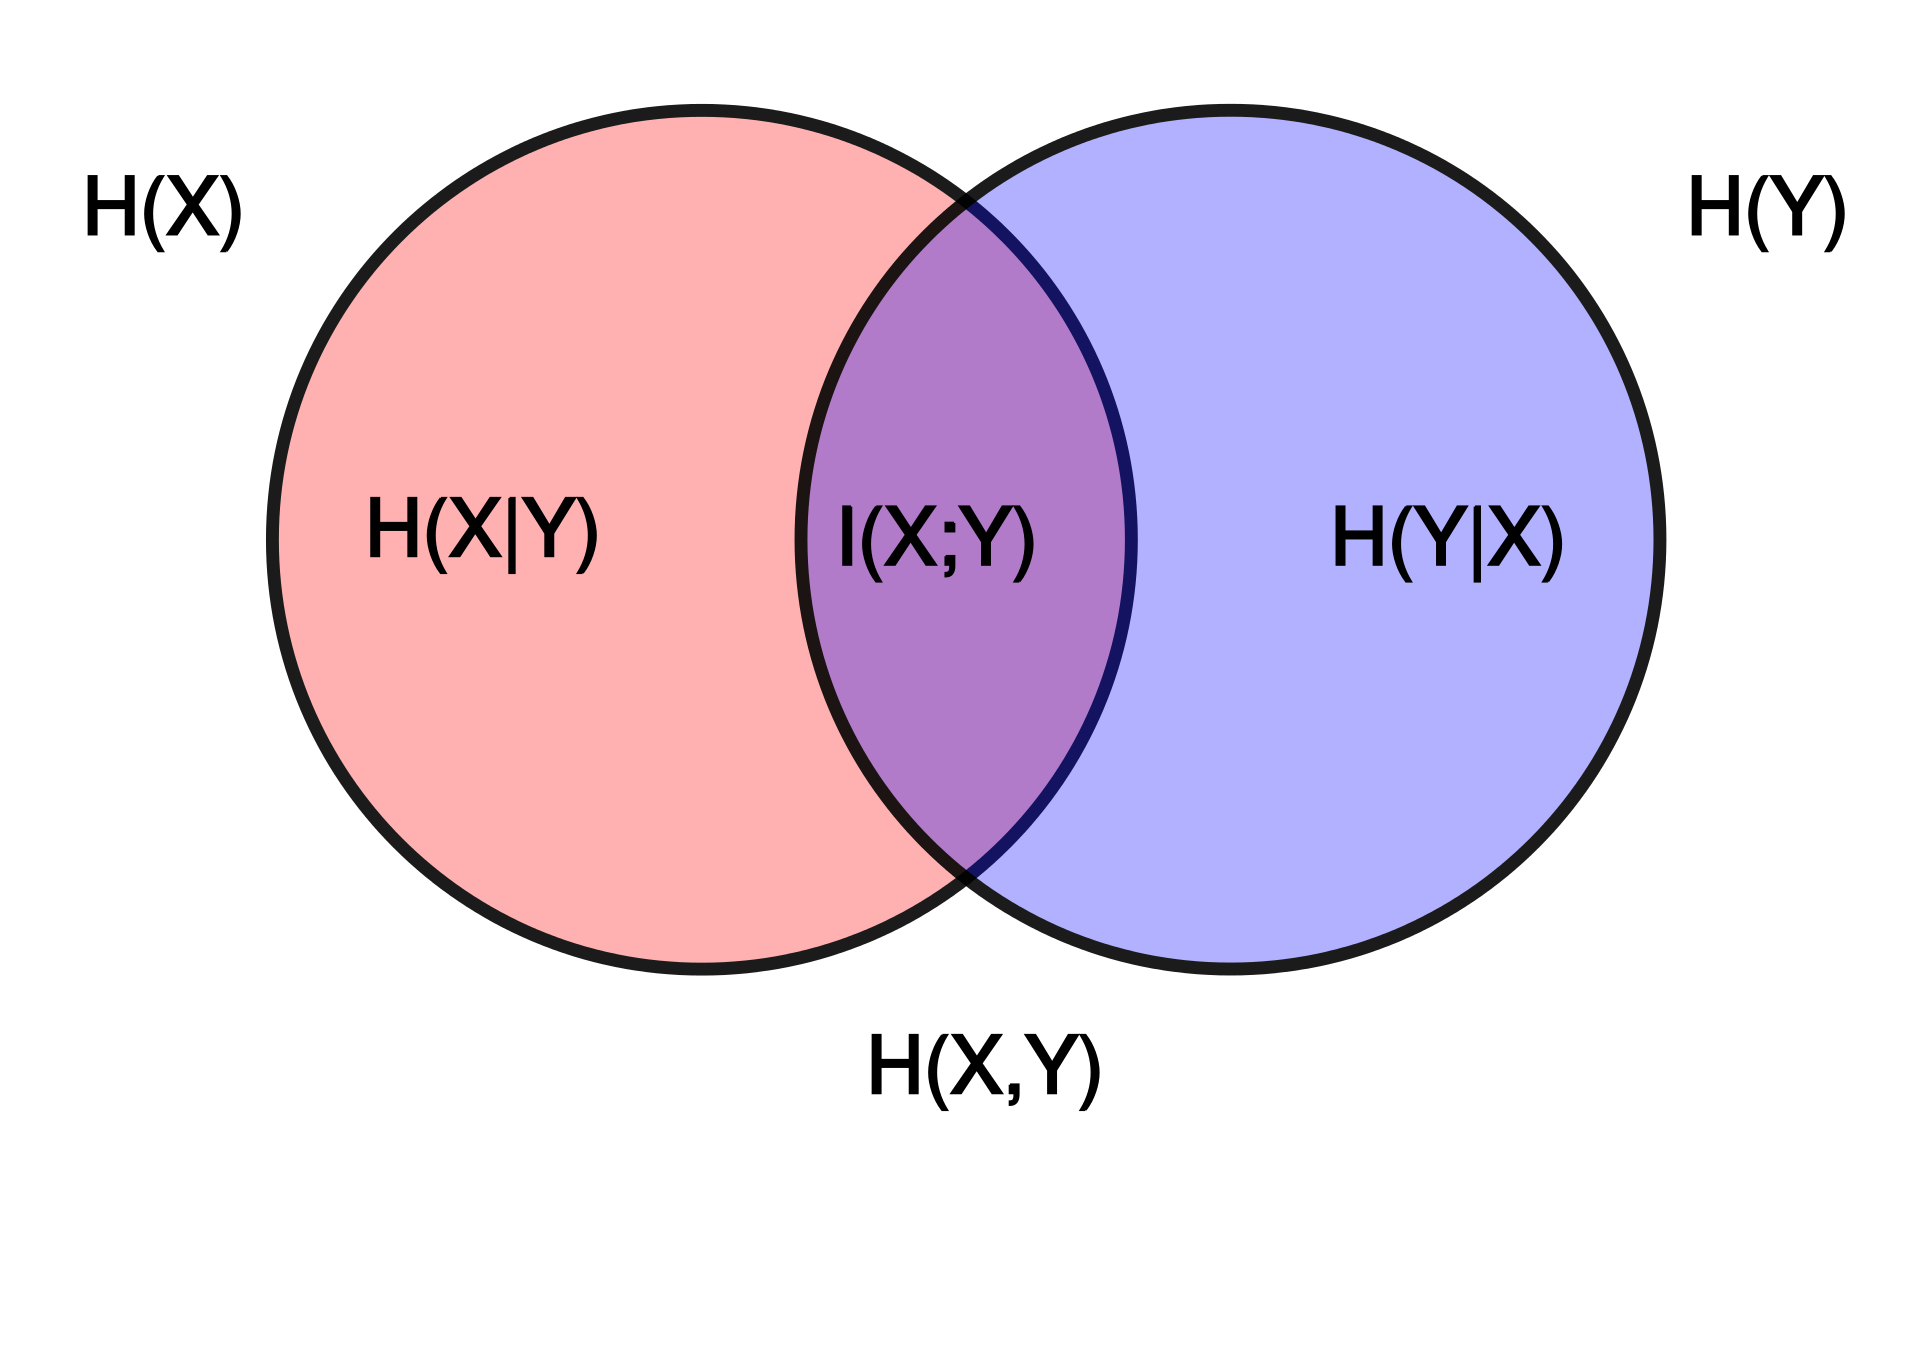
\includegraphics[width=0.7\textwidth]{includes/figures/defi_information_gain.png}
    \end{center}

    Information Gain wird von den Algorithmen \emph{ID3}, \emph{C4.5} und \emph{C5.0} genutzt.
\end{defi}

\begin{example}{Mutual Information}
    \begin{center}
        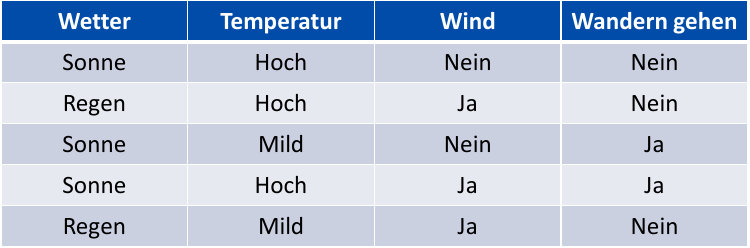
\includegraphics[width=0.6\textwidth]{includes/figures/example_information_gain.png}
    \end{center}

    % \begin{enumerate}[a)]
    %     \item Bestimmen Sie die Entropie für \enquote{Wandern gehen} (und geben Sie ihren Wert hier an).
    %     \item Bestimmen Sie die bedingten Entropien für \enquote{Wandern gehen} bezüglich der Features und geben Sie die Werte, die Sie erhalten haben, an.
    %     \item Bestimmen Sie den Information Gain für jedes Feature und geben sie die Werte hier an.
    % \end{enumerate}

    % \exampleseparator

    a) Bestimmen Sie die Entropie für \enquote{Wandern} (und geben Sie ihren Wert hier an).
    \[
        H(X) = - \sum_{k=1}^{C} p_k \log_2 p_k = - p_1 \log_2 p_1 - p_2 \log_2 p_2 = \frac{2}{5} \cdot \log_2 \frac{2}{5} - \frac{3}{5} \cdot \log_2 \frac{3}{5} \approx 0.97
    \]

    b) Bestimmen Sie die bedingten Entropien für \enquote{Wandern} bezüglich der Features und geben Sie die Werte, die Sie erhalten haben, an.
    \[
        H(Y \mid X) = - \sum_j p(x_j) \left( \sum_i p(y_i \mid x_j) \log_2 p(y_i \mid x_j) \right)
    \]

    Damit gilt:
    \[
        H(\text{Wandern} \mid \text{Wetter})
        = - \underbrace{\frac{3}{5} \left( \underbrace{\frac{2}{3} \log_2 \frac{2}{3}}_{\text{Wandern Ja}} + \underbrace{\frac{1}{3} \log_2 \frac{1}{3}}_{\text{Wandern Nein}} \right)}_{\text{Sonne}}
        - \underbrace{\frac{2}{5} \left( \underbrace{\frac{0}{2} \log_2 \frac{0}{2}}_{\text{Wandern Ja}} + \underbrace{\frac{2}{2} \log_2 \frac{2}{2}}_{\text{Wandern Nein}} \right)}_{\text{Regen}}
        \approx 0.55
    \]
    \[
        H(\text{Wandern} \mid \text{Temp.})
        = - \underbrace{\frac{3}{5} \left( \underbrace{\frac{1}{3} \log_2 \frac{1}{3}}_{\text{Wandern Ja}} + \underbrace{\frac{2}{3} \log_2 \frac{2}{3}}_{\text{Wandern Nein}} \right)}_{\text{Hoch}}
        - \underbrace{\frac{2}{5} \left( \underbrace{\frac{1}{2} \log_2 \frac{1}{2}}_{\text{Wandern Ja}} + \underbrace{\frac{1}{2} \log_2 \frac{1}{2}}_{\text{Wandern Nein}} \right)}_{\text{Mild}}
        \approx 0.95
    \]
    \[
        H(\text{Wandern} \mid \text{Wind})
        = - \underbrace{\frac{3}{5} \left( \underbrace{\frac{1}{3} \log_2 \frac{1}{3}}_{\text{Wandern Ja}} + \underbrace{\frac{2}{3} \log_2 \frac{2}{3}}_{\text{Wandern Nein}} \right)}_{\text{Wind Ja}}
        - \underbrace{\frac{2}{5} \left( \underbrace{\frac{1}{2} \log_2 \frac{1}{2}}_{\text{Wandern Ja}} + \underbrace{\frac{1}{2} \log_2 \frac{1}{2}}_{\text{Wandern Nein}} \right)}_{\text{Wind Nein}}
        \approx 0.95
    \]

    c) Bestimmen Sie die Mutual Information für jedes Feature und geben sie die Werte hier an.
    \[
        \text{IG}(Y, X) = H(Y) - H(Y \mid X)
    \]

    Damit gilt:
    \[
        \text{IG}(\text{Wandern}, \text{Wetter}) = H(\text{Wandern}) - H(\text{Wandern} \mid \text{Wetter})
        = 0.97 - 0.55 = 0.42
    \]
    \[
        \text{IG}(\text{Wandern}, \text{Temperatur}) = \ldots
        = 0.97 - 0.95 = 0.02
    \]
    \[
        \text{IG}(\text{Wandern}, \text{Wind}) = \ldots
        = 0.97 - 0.95 = 0.02
    \]
\end{example}

\begin{bonus}{Korrelation und Kausalität}
    Hohe Werte von Zusammenhangsmaßen können hindeuten auf kausale Zusammenhänge, diese aber nicht begründen.

    Kontrollierte Experimente können zur Entdeckung von kausalen Zusammenhängen genutzt werden.
    Typisch: Merkmal $X$ wird im Experiment verändert, und man beobachtet die daraus resultierenden oder nicht resultierenden Änderungen von Merkmal $Y$.

    Experimente lassen sich aber in vielen Fällen nicht realisieren.\footnote{Dieser Umstand begründet die Entwicklung von Maßen zur Charakterisierung der Richtung eines Zusammenhangs (z.B. \emph{Granger Causality})}
\end{bonus}

\subsection{Interpretationsfehler}

\begin{defi}{Scheinkausalität}
    Eine \emph{Scheinkausalität} ist eine Korrelation, die nicht mit einem kausalen Zusammenhang assoziiert ist.

    Es gibt drei Typen von Scheinkausalität:
    \begin{itemize}
        \item \emph{Common Driver}: Ein drittes Merkmal $X$, das mit $Y$ und $Z$ hochkorreliert ist, blieb in der Analyse zunächst unberücksichtigt.
              Wir beobachten also eine Scheinkorrelation zwischen $Y$ und $Z$.

              \begin{center}
                  \includegraphics[width=.5\textwidth]{includes/figures/example_common_driver.pdf}
              \end{center}
        \item \emph{Indirekte Beziehung}:

              \begin{center}
                  \includegraphics[width=.5\textwidth]{includes/figures/example_indirekte_beziehung.pdf}
              \end{center}
        \item \emph{Zufällige Korrelation}:

              \begin{center}
                  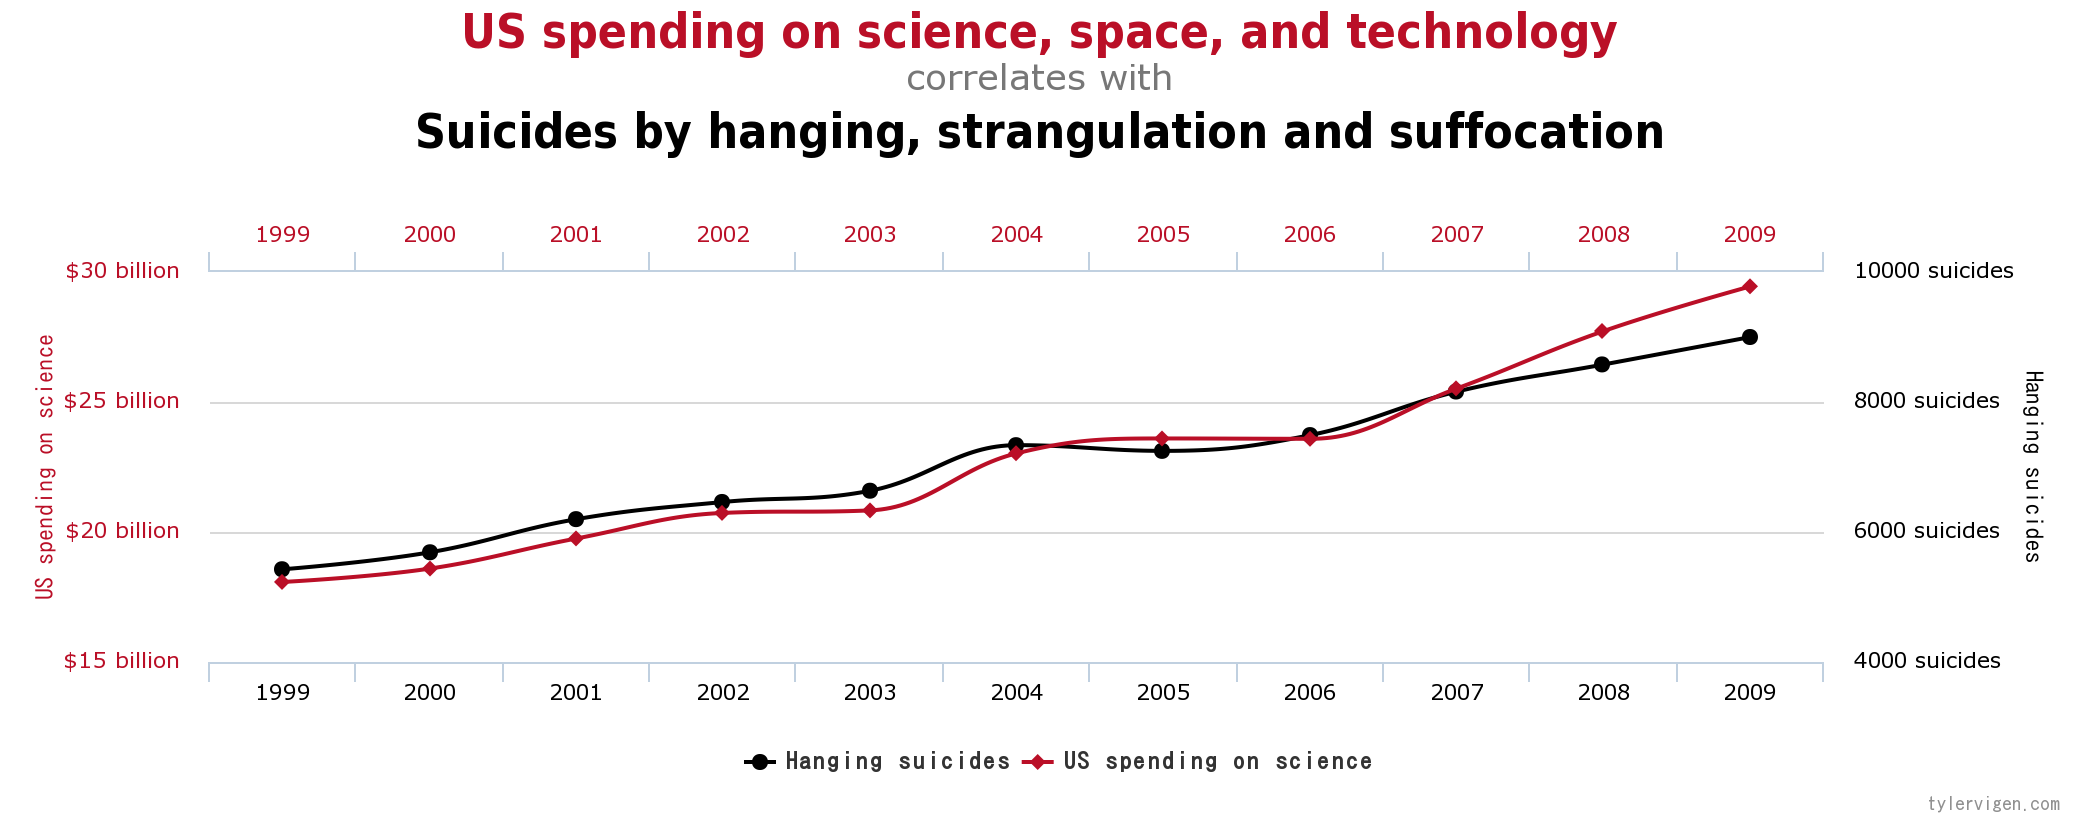
\includegraphics[width=.9\textwidth]{includes/figures/example_zufaellige_korrelation.png}
              \end{center}
    \end{itemize}


\end{defi}

\begin{defi}{Verdeckte Korrelation}
    Von einer \emph{verdeckten Korrelation} spricht man, wenn statistisch keinerlei Korrelation errechnet wurde, obwohl sachlich eindeutig Zusammenhänge vorliegen.

    Verdeckte Korrelation kann auftreten, wenn eine Population in Teilpopulationen zerfällt.
\end{defi}
